\documentclass[a4paper]{article}

%% Language and font encodings
\usepackage[english]{babel}
\usepackage[utf8x]{inputenc}
\usepackage[T1]{fontenc}

%% Sets page size and margins
\usepackage[a4paper,top=3cm,bottom=2cm,left=3cm,right=3cm,marginparwidth=1.75cm]{geometry}

%% Useful packages
\usepackage{amsthm}
\usepackage{amsmath}
\usepackage{amssymb}
\usepackage{graphicx}
\usepackage[colorinlistoftodos]{todonotes}
\usepackage[colorlinks=true, allcolors=blue]{hyperref}
\usepackage{mathabx}
\usepackage{tikz}

\setlength\parindent{0pt}

\title{CS 4780/5780 Homework 7\vspace{-10pt}}
% \author{Due: Tuesday 04/10/18 11:55pm on Gradescope}
\date{\vspace{-0pt}}

\begin{document}
\maketitle

\subsection*{Problem 1: Derivation for Hard-margin Linear SVMs}
\textbf{a)} Suppose your data is linearly separable. Why might you prefer the hard-margin linear SVM solution over the solution found by the Perceptron?\\

The hard-margin linear SVM solution gives the "best" separating hyperplane, i.e. the one that maximizes the margin to the nearest data points, whereas the perceptron gives any seperating hyperplane.

\textbf{b)} The most intuitive definition of the hard-margin linear SVM is to "maximize the margin of the hyperplane, subject to the constraint that every training point is classified correctly." Write this objective mathematically, and label which parts of your formulation correspond to each part of our intuitive definition. (Hint: it's in the notes.)\\

$\min_{w,b}\frac{1}{\lVert w \rVert_2} \min_{x_i \in D} |w^Tx_i + b|$ [Maximize the margin of the hyperplane]\\
s.t. $\forall i, y_i(w^Tx_i + b) \geq 0$ [Every training point is classified correctly]\\

\textbf{c)} Though the maximum margin separating hyperplane is unique, the $(\mathbf{w},b)$ we use to define it is not unique unless we do something like restrict the norm of $\mathbf{w}$. That's precisely what we do when we include the constraint $\min_i\|\mathbf{w}^\top\mathbf{x}_i+b\|=1$. What have we restricted $\|\mathbf{w}\|_2$ to equal? (Hint: recall the definition of the margin of a hyperplane.)\\

$\min_i\|\mathbf{w}^\top\mathbf{x}_i+b\|=1 \implies \lVert \mathbf{w} \rVert_2\Bigg(\min_i\dfrac{\|\mathbf{w}^\top\mathbf{x}_i+b\|}{\lVert \mathbf{w} \rVert_2}\Bigg)=1 \implies \lVert \mathbf{w} \rVert_2(margin)=1 \implies \boxed{\lVert \mathbf{w} \rVert_2 = \frac{1}{\gamma}}$

\textbf{d)} At this point we can do some quick algebra to get the following formulation:
\begin{align*} &\min_{\mathbf{w},b} \mathbf{w}^\top\mathbf{w} & \\ &\textrm{s.t. } \begin{matrix} \forall_i \ y_{i}(\mathbf{w}^T \mathbf{x}_{i}+b)&\geq 0\\ \min_{i}\left | \mathbf{w}^T \mathbf{x}_{i}+b \right | &= 1 \end{matrix} \end{align*}
Prove that for the optimal solution, these constraints are equivalent to $ \forall_i \ y_{i}(\mathbf{w}^T \mathbf{x}_{i}+b) \geq 1 $.\\

In the optimal solution, all the points are classified correctly and these constraints are satisfied. Since $y_i \in \{-1,+1\}$, and $|w^Tx_i+b| \geq 1$ for all data points $x_i$, we can multiply $|y_i|$ by $|w^Tx_i+b|$ to get the single constraint $|y_i(w^Tx_i+b)| \geq 1$. However, using the fact that $\forall_i \ y_{i}(\mathbf{w}^T \mathbf{x}_{i}+b) \geq 1$, we can remove the absolute value and get $y_i(w^Tx_i+b) \geq 1$.\\

\subsection*{Problem 2: Hard- vs. Soft-margin SVMs}
\textbf{a)} The Perceptron algorithm does not converge on non-linearly separable data. Does the hard-margin SVM converge on non-linearly separable data? How about the soft-margin SVM? Why?\\

The hard-margin SVM does not converge on non-linearly separable data but the soft-margin SVM does because the soft constraints introduce a slack variable which allows the initial constraints presented in the hard-margin version to be violated such that the optimization problem becomes solvable. \\

\textbf{b)} For the soft-margin linear SVM, we use the hyperparameter $C$ to tune how much we penalize misclassifications. As $C\rightarrow\infty$, does the soft-margin SVM become more similar or less similar to the hard-margin SVM? As $C\rightarrow 0^+$, what happens to the solution of the soft-margin SVM? Why?\\

As $C\rightarrow\infty$, the soft-margin SVM becomes more similar to the hard margin SVM. As $C\rightarrow0^+$, the soft-margin SVM completely ignores the data. This is because $C$ represents the penalty for misclassifying a training point. \\

\textbf{c)} How would \textit{you} go about picking a good value for $C$? \\

One way would be to split the training set into a validation set in order to compare different values for $C$. This could involve applying a telescopic search on $C$ values which will be covered in more detail in a later lecture. Of course, all of these decisions would depend on your confidence in the regularization within the context of the problem. In general, more noisy data will require more slack than a less noisy data set.\\

\subsection*{Problem 3: Thinking in Terms of the "Buffer"}
\textbf{a)} Suppose you found a solution $(\mathbf{\hat w},\hat b)$ to the hard-margin SVM. The separating hyperplane is surrounded by a buffer defined by hyperplanes $\{\mathbf{x}: \mathbf{\hat w}^\top\mathbf{x}+\hat b=1\}$ and $\{\mathbf{x}: \mathbf{\hat w}^\top\mathbf{x}+\hat b=-1\}$. Prove that at least one training datapoint lies on each of these buffer hyperplanes.\\

\[
\min_{x \in D} |\mathbf{\hat w}^\top\mathbf{x} + \hat b| = 1 \\
\implies \exists x \text{ s.t. } \mathbf{\hat w}^\top\mathbf{x} + \hat b = 1 \text{ OR } \mathbf{\hat w}^\top\mathbf{x} + \hat b = -1
\] \\

This only shows that at least on training datapoint lies on at least one of the two buffer hyperplanes. \\

Now, let us proceed with the assumption that there is no point on one of the two buffer hyperplanes. If this was the case, then the solution to the maximum margin optimization would yield different buffer hyperplanes. This contradicts the given buffer hyperplanes in the problem and so there must be at least one training datapoint on \textbf{each} hyperplane. \\

\textbf{b)} Your TA is unimpressed with your solution and says you didn't minimize $\|\mathbf{w}\|_2$ enough, so he tells you to use $(\mathbf{w}_{TA},b_{TA})=(0.9*\mathbf{\hat w},0.9*\hat b)$. Prove that, though this solution corresponds to the same hyperplane, it has violated a constraint in the hard-margin SVM optimization problem. What happened to the buffer, when you rescaled (decreased) the norm of the solution?\\

The constraint that $\min_{x \in D} |\mathbf{\hat w}^\top\mathbf{x} + \hat b| = 1$ is no longer satisfied and the buffer has decreased. \\

\textbf{c)} Your TA doesn't understand your proof, so you decide to give him a pictorial explanation. Draw a reasonable, linearly separable, binary class, 2D dataset. Draw the hyperplane and buffer corresponding to the hard-margin SVM solution $(\mathbf{\hat w},\hat b)$ for this dataset. Then on another plot, roughly draw the hyperplane and buffer corresponding to the TA's scaled version, $(\mathbf{w}_{TA},b_{TA})=(0.9*\mathbf{\hat w},0.9*\hat b)$.\\

\begin{center}
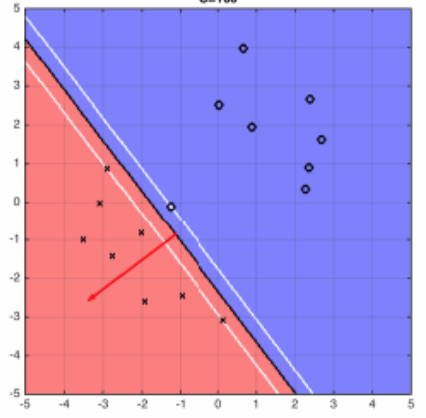
\includegraphics{SVM.png}
\end{center}
In the TA's scaled version, the margins would be moved further from the hyperplane, leaving at least two datapoints in between the buffers.\\

\textbf{d)} Your TA is embarrassed, so you graciously say that he obviously meant that you should use a soft-margin SVM. Why is $(\mathbf{w}_{TA},b_{TA})$ now, in the case of soft-margin SVMs, a reasonable suggestion? Are training datapoints "allowed past the buffer" for soft-margin SVMs? \\

$(\mathbf{w}_{TA},b_{TA})$ is reasonable because it doesn't violate any constraints as it does for the hard-margin (shown in (b)) while giving a 'simpler' solution and because the training datapoints are "allowed past the buffer" for soft-margin SVMs.


\subsection*{Problem 4: MLE in terms of ERM}
Recall that a generative model assigns a probability to every features-label pair $(x,y)$. Suppose that we would like to learn a generative model $g$. What constitutes a "good" $g$? In class you have discussed a few learning principles. In this problem, you will show that there is a cool connection between MLE, ERM with a particular loss function, and minimizing the KL-divergence. First, some background:\\

The KL-divergence is a measure of how much the distribution $p$ diverges from the distribution $q$. It is defined as $$D_{KL}(p||q) = \mathbb{E}_{(x,y)\sim p} \left[\log\frac{p(x,y)}{q(x,y)}\right].$$

True risk is defined as the expected loss of your classifier, $\mathbb{E}_{(x,y)\sim\pi} \left[\ell(h(x),y)\right]$ -- where $\pi$ is the true test-time distribution, $\ell$ is the loss function of interest, and $h$ is the learned function. Ideally, we would learn a function which minimizes the true risk $$\hat h = \arg\min_h \mathbb{E}_{(x,y)\sim\pi} \left[\ell(h(x),y)\right].$$ We usually can't evaluate this directly because we don't know $\pi$. Instead, we consider the empirical risk, $\sum_{(x,y)\in D}\ell(h(x),y)$ -- where $D$ is a training dataset of examples. If $D$ is large and drawn iid from $\pi$, then the empirical risk approaches the true risk. In ERM, our learning algorithm attempts to find a function $\hat h$ which minimizes the empirical risk $$\hat h = \arg\min_h \sum_{(x,y)\in D}\ell(h(x),y).$$\\

\textbf{a)} Suppose our learning goal is to minimize the KL-divergence from our model distribution to the true data distribution, $$\hat g = \arg\min_g \mathbb{E}_{(x,y)\sim\pi} \left[\log\frac{\pi(x,y)}{g(x,y)}\right].$$ Show that this is, in fact, a type of true risk minimization. In particular: what is the predictive function $h$? what is the loss function $\ell$?\\

\begin{align*}
    \hat{g} &= \arg\min_g \mathbb{E}_{(x,y)\sim\pi}\left[\log\frac{\pi(x,y)}{g(x,y)}\right] \\
    &= \arg\min_g \mathbb{E}_{(x,y)\sim\pi}\left[\log\pi(x,y) - \log g(x,y)\right] \\
    &= \arg\min_g \mathbb{E}_{(x,y)\sim\pi}\left[- \log g(x,y)\right] \\
\end{align*}

Thus, 
$$h(x) = g(x,*)$$
which uses currying and $h(x)$ is a function of $y$. It outputs a probability disribution, not a point estimation. 

Then the loss function is (cross-entropy loss): 
$$l = -\log (g(x,y)) = -\log( h(x)(y))$$

\textbf{b)} What is the empirical risk minimization problem, for the true risk minimization problem you defined in part (a)?\\

$$\hat{g} = \text{arg min}_g \sum_{(x,y)\in D} -\log(g(x,y))$$

\textbf{c)} Show that the solution to the empirical risk minimization problem is equivalent to the solution to the maximum likelihood optimization problem $$\hat g = \arg\max_g \prod_{(x,y)\in D} g(x,y).$$

\begin{align*}
   \hat{g} &= \arg\min_g \sum_{(x,y)\inD} -\log(g(x,y))\\
   &= \arg\max_g\sum_{(x,y)\in D} \log(g(x,y))\\
   &= \arg \max_g \prod_{(x,y)\in D} g(x,y)
\end{align*}

\end{document}
